%!TEX root = syntheyes15.tex

\section{Synthetic data generation}

\cite{MIL-STD-1472G} -- cite for range of eye rotation.

\begin{figure}
    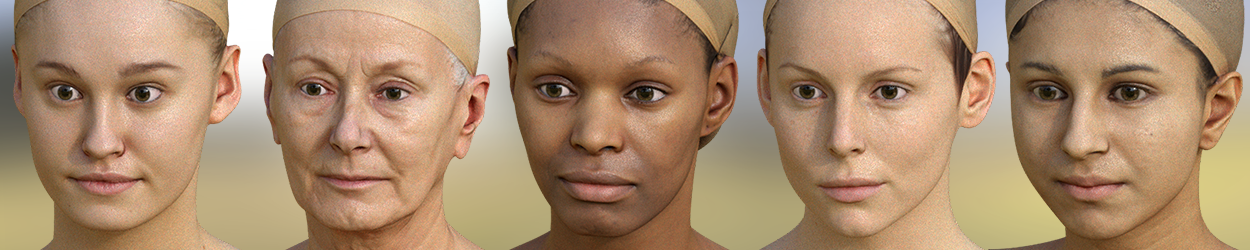
\includegraphics[width=\columnwidth]{participants_f} \par \smallskip
    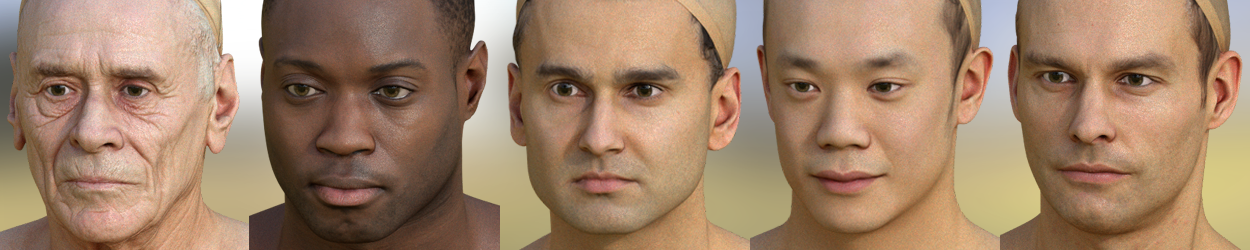
\includegraphics[width=\columnwidth]{participants_m}
    \caption{Our suite of female and male head models for rendering.}
    \label{fig:participants}
\end{figure}

\begin{figure}
    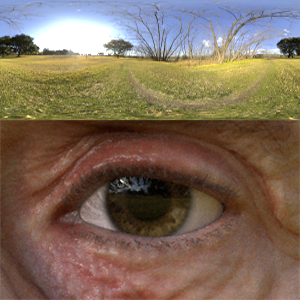
\includegraphics[width=0.24\columnwidth]{fig_env_1} \hfill
    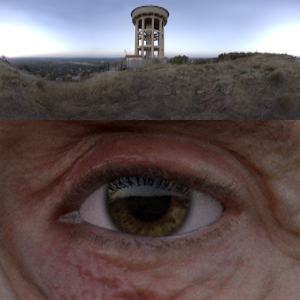
\includegraphics[width=0.24\columnwidth]{fig_env_2} \hfill
    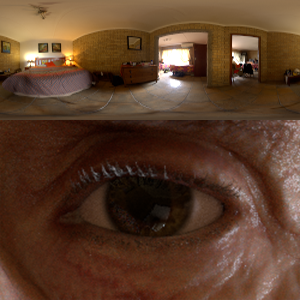
\includegraphics[width=0.24\columnwidth]{fig_env_3} \hfill
    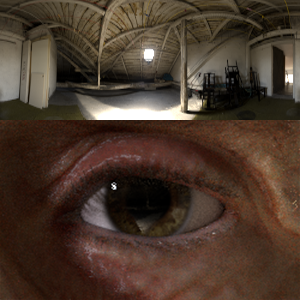
\includegraphics[width=0.24\columnwidth]{fig_env_4}
    \caption{Appearance variation from lighting is modelled with poseable high-dynamic-range environment maps \cite{debevec2002image}.}
    \label{fig:participants}
\end{figure}

\subsection{Eye model}

\begin{figure}
    \centering
    \begin{subfigure}[t]{0.33\columnwidth}
        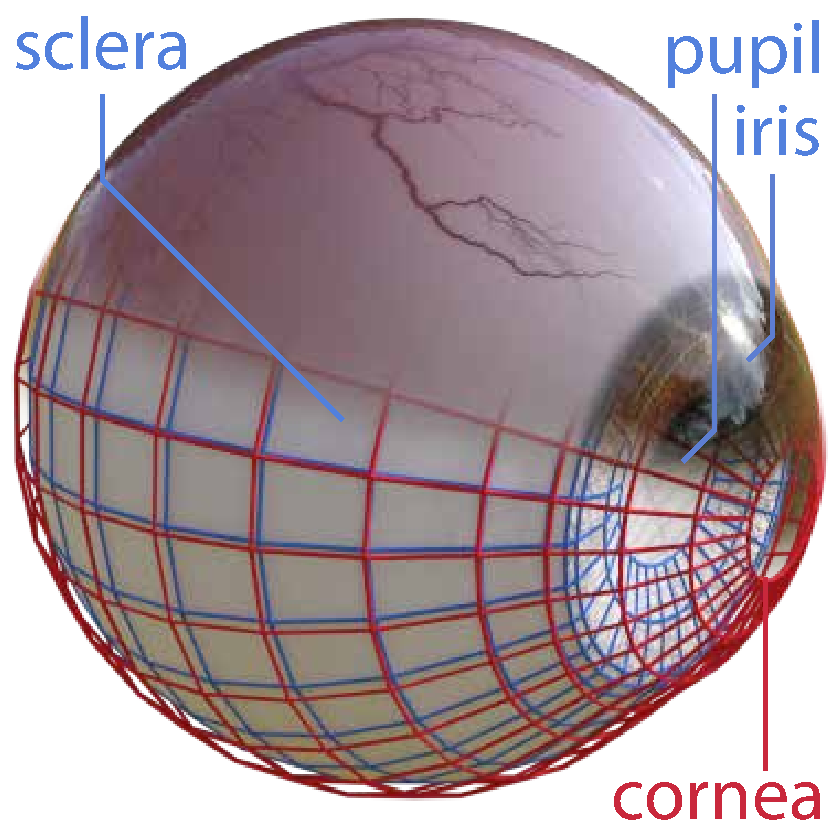
\includegraphics[width=\textwidth]{eye_model}
        \caption{3D eye model}
        \label{fig:3d_eye_model}
    \end{subfigure}%
    \hfill
    \begin{subfigure}[t]{0.65\columnwidth}
        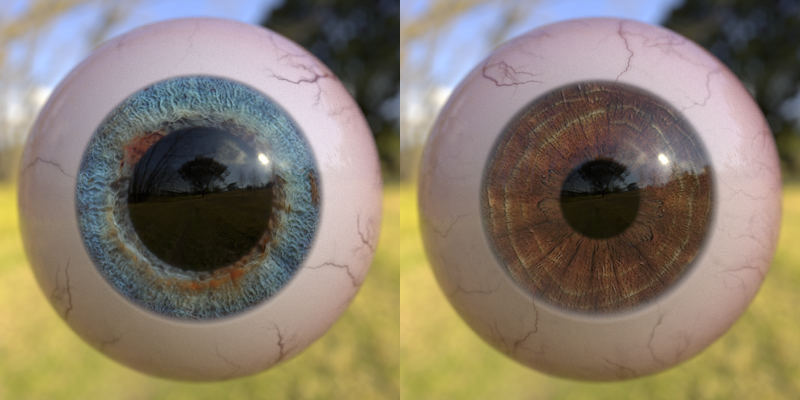
\includegraphics[width=\textwidth]{eye_examples}
        \caption{Pupil dilation and iris color variation}
    \end{subfigure}
    \caption{Our realistic eye model is capable of expressing degrees of variability seen in real life.}
    \label{fig:eye_model}
\end{figure}

Eyeballs are complex organs comprised of multiple layers of tissue, each with different reflectance properties and levels of transparency. Fortunately, as realistic eyes are so important for many areas of CG, there is already a large body of previous work on modelling and rendering eyes \commentE{cite}.

% It is important to accurately model reflections and refractions in the eye as they can lead to specular highlights -- these common eye-region image features are often used by eye-tracking algorithms, or can confound approaches that are not robust.

As shown in \autoref{fig:3d_eye_model}, our eye model consists of two parts.
%
The outer part (red wireframe) approximates the eye's overall shape with two spheres ($r_1\!=\!12\textrm{mm}, r_2\!=\!8\textrm{mm}$ \cite{ruhland2014look}), the latter representing the corneal bulge. To avoid a discontinuous seam between spheres, the meshes were joined and then smoothed. It is transparent, refractive ($n\!=\!1.376$), and partially reflective. The eye's bumpy surface variation is modelled by a displacement map generated with noise functions.
%
The inner part (blue wireframe) is a flattened sphere with Lambertian material. The planar end represents the iris and pupil, and the rest represents the sclera -- the white of the eye.
%
There is a $0.5\textrm{mm}$ gap between the outer and inner parts which accounts for the thickness of the cornea.

Eyes exhibit variations in both shape (pupillary dilation) and texture (iris color and scleral veins). To model shape variation we use \emph{shape keys} -- 

To model how iris color varies between people, we 

Iris color varies between people, and it is important for us to model this.

Previous research on iris-synthesis 

Photo-textures were used for the irises

\subsection{Eye-region model suite}

\subsection{Eyelid motion}

Vertical saccades are always accompanied by eyelid motion \cite{liversedge2011oxford}.